\documentclass[12pt]{article}
\usepackage[utf8]{inputenc}
\usepackage[english]{babel}

\usepackage[a4paper, margin=1in]{geometry}

\usepackage[usenames, dvipsnames]{color}
\usepackage[parfill]{parskip}

\usepackage{graphicx}
\graphicspath{ {images/} }

\usepackage{minted}
\usepackage{mdframed}
\surroundwithmdframed{minted}

\usepackage{fancyhdr}
\pagestyle{fancy}
\fancyhf{}
\rhead{Session 1 and 2}
\lhead{Workshop: Text Analysis and Word Vectors in R}
\rfoot{Page \thepage}
\lfoot{Sara J Kerr. Frankfurt - Jan 2017}

\renewcommand{\headrulewidth}{0.4pt}
\renewcommand{\footrulewidth}{0.4pt}
\usepackage{hyperref}
\hypersetup{
    colorlinks=true,
    linkcolor=RoyalPurple,     
    urlcolor=RoyalPurple,
}
 
\urlstyle{same}

\title{{Text Analysis and Word Vectors in R} \\ {Workshop at Goethe University Frankfurt}  \newline }
\author{Sara J Kerr M.A.\thanks{PhD Candidate at An Foras Feasa, Maynooth University, Ireland. \newline Supported by a Pat and John Hume Scholarship.}} 
\date{25th January 2017}


\begin{document}

\setlength{\parindent}{0pt}
\setlength{\parskip}{1em}

\begin{titlepage}
\maketitle
\end{titlepage}

\tableofcontents

\section*{Overview}
This workshop will provide an introduction to textual analysis and word vector analysis in R.  R is a free and open source piece of software traditionally used for statistical analysis. Packages for R can be installed from the CRAN website, via R Studio, or directly from a source website.

The workshop aims to introduce textual analysis and word vectors using R and provide a starting point for further exploration. The materials used will be examples from Jane Austen's works. Session 1 will explore some basic text analysis using R, in particular frequency analysis and Key Word in Context. While these are not necessary for using word vectors, they are helpful for putting the results of the vector space model into context and allow exploration at text level.

To apply the analysis in Workshop Session One to Japanese the chosen texts will need to be split into words using a package like \textbf{RMeCab} (which can be found \href{http://rmecab.jp/wiki/index.php?RMeCab}{\textbf{here}}) as the function used to separate the texts into word lists relies upon an regular expression and gaps between words. Unfortunately I can't give further instructions on the use of this package as the website is in Japanese. Another useful package is \textbf{Nippon} which includes a variety of utilities for handling Japanese text, including converting text from Katakana to Hiragana. 

For more advanced exploration of texts there is \textbf{Stylo}, a package for stylometric analysis, which has options for use with Chinese and Japanese text. For further information about the \textbf{Stylo} package see \href{https://cran.r-project.org/web/packages/stylo/stylo.pdf}{\textbf{Stylo}}, \href{https://journal.r-project.org/archive/accepted/eder-rybicki-kestemont.pdf}{\textbf{Stylometry with R}}, or \href{https://my.vanderbilt.edu/digitalhumanities/using-r-for-stylometric-analysis-with-the-stylo-package/}{\textbf{Using R for Stylometric Analysis}}.


\section{Workshop Session One: Text Analysis in R}

Session 1, subsections 1--4 are adapted from Matthew L. Jockers (2014) \textit{\textbf{Text Analysis with R for Students of Literature}}.

Session 1, subsection 5 is adapted from \href{https://eight2late.wordpress.com/2015/05/27/a-gentle-introduction-to-text-mining-using-r/}{\textbf{A gentle introduction to text mining using R}}.

You will need to to to \textbf{\url{https://sarajkerr.com/workshops/}} and download the resources you need for the workshop.  When creating folder names it is important that they do not contain any gaps as this can cause problems when accessing them from R Studio. Your Workshop folder should have the following structure:

\begin{figure}[H]
	\centering
	\includegraphics[width=0.75\textwidth]{workshop.jpg}
	\caption{The Workshop Folder}
\end{figure}


Open R Studio.

Before you start you need to set your `working directory', this is the folder where the texts and results are stored. Go to \textit{Session} - \textit{Set Working Directory} - \textit{Choose Directory} then browse to the folder \textit{Workshop} on your desktop.

\begin{figure}[H]
	\centering
	\includegraphics[width=0.75\textwidth]{setdir.jpg}
	\caption{Setting the Working Directory}
\end{figure}
 
 You will notice that a piece of code has appeared in the R console:
\medskip
 \begin{minted}
[fontsize=\footnotesize,
linenos
]
{r}  
setwd("pathway to the working directory")

# This is the function that sets the working directory
\end{minted}

This first section focuses on frequency analysis using base R.  

\subsection{Load and Preprocess a File}

To load the first file and view the first 6 elements: 
\medskip
\begin{minted}
[fontsize=\footnotesize,
linenos
]
{r} 
ja_ch <- scan("Austen_Texts/Chapter_Files/PP1_En.txt", what = "character", 
              sep = "\n")

# This can also be done using
mytext <- scan(file.choose(), what ="character", sep = "\n") 
# which allows you to search for the file you want

# A character file has been created with 80 elements.

head(ja_ch)
\end{minted}

The output will show the first 6 lines of the document - in this case the title and first 4 lines of Chapter 1 of Jane Austen's \textit{Pride and Prejudice}. Each line is enclosed in speech marks as they are character strings. You will also notice that a value \textbf{ja{\_}ch} is now in the environment pane, each time you create something it will appear in this pane. This is a character (chr) vector which has 80 elements. To access an individual element or a selection of elements:
\medskip
\begin{minted}
[fontsize=\footnotesize,
linenos
]
{r} 
ja_ch[1]
ja_ch[3:4]
\end{minted}

Now create a new vector which only contains the chapter text:
\medskip
\begin{minted}
[fontsize=\footnotesize,
linenos
]
{r} 
ja_ch1 <- ja_ch[3:80]
# Check the first 6 lines 
head(ja_ch1)
\end{minted}

Load the second chapter \textbf{PP1{\_}De.txt} into a vector called \textbf{ja{\_}ch{\_}d}. Create a vector which removes the first two lines and saves the chapter text into a new vector called \textbf{ja{\_}ch1d}. You should now have a character vector which contains a bad German translation of the first chapter of \textit{Pride and Prejudice} (thanks to Google Translate).  

Remove line breaks from each file (if you wish to start over in the same session rerun these two lines of code to recreate the unprocessed text). It is a good idea to keep a vector of the text in an unprocessed form, if you make a mistake you won't have to start from the beginning.
\medskip
\begin{minted}
[fontsize=\footnotesize,
linenos
]
{r} 
text1 <- paste(ja_ch1, collapse = " ")
text2 <- paste(ja_ch1d, collapse = " ")
\end{minted}

The chapters are each now a single character string.

Before word frequencies can be calculated, the text needs to be processed. The level of processing will depend on the text and its language. For the texts we are using we will change the text to lower case, and extract the words saving them as a vector .
\medskip
\begin{minted}
[fontsize=\footnotesize,
linenos
]
{r} 
# Change text to lower case
text1 <- tolower(text1) 
# Check in the environment pane - the capital letters have now been removed

# select words only
text1 <- strsplit(text1, "\\W") # The second argument is a regular expression

# If we look in the environment pane text1 is now a 'List of 1'
text1 <- unlist(text1) # simplify to a vector
text1
\end{minted}

Most of the chapter is now displayed (R 	has a `maximum print' limit), but where there was punctuation there are now ``'' indicating an empty space. Our next step is to remove these.
\medskip
\begin{minted}
[fontsize=\footnotesize,
linenos
]
{r} 
text1 <- text1[which(text1 != "")] # '!=' means 'does not equal'
# This subsets the vector by removing elements which are not spaces
text1
\end{minted}

\textbf{text1} is now a character vector where each word is an element. If we look at the environment pane we can see the length of the vector in square brackets - 852. This gives us the number of tokens (words) in the text. It is also possible to calculate the length of a vector directly in R:
\medskip
\begin{minted}
[fontsize=\footnotesize,
linenos
]
{r} 
length(text1)
\end{minted}

Now do the same for \textbf{text2}.

\subsection{Tokens, Types and Word Frequency}

You can search for a word by its index number - R starts indexing at 1 - or by using the \textbf{which()} function. The \textbf{which()} function will return the index numbers of all occurrences of the selected word. By using the \textbf{length()} function we can identify how many times a word appears in the text. We can also use the \textbf{unique()} function to identify the word types in the text.
\medskip
\begin{minted}
[fontsize=\footnotesize,
linenos
]
{r} 
text1[42]
text2[723]

which(text1 == "neighbourhood")
which(text2 == "nachbarschaft")

# number of times a word appears in the text
length(text1[which(text1 == "neighbourhood")])

# number of types in the text
length(unique(text2))
\end{minted}

Now we will use R to create a raw frequency table, sort it by most frequent words and view the top 10 as a list and as a simple plot. 
\medskip
\begin{minted}
[fontsize=\footnotesize,
linenos
]
{r} 
# create a table of frequencies
text1_freqs <- table(text1)

# sort by frequency
sorted_text1 <- sort(text1_freqs, decreasing = TRUE)

# View the top 10 most frequent words in the text
sorted_text1[1:10]

# View as a plot
plot(sorted_text1[1:10])
# If all 10 words don't appear click on the Zoom option in the plot pane.
\end{minted}

Although it can be interesting to view the raw frequencies, calculating the relative frequencies allows for comparisons to be made across and between texts. The code below calculates the relative frequencies and plots the top ten words. This time we are going to add a title to the plot and custom x and y-axis titles. 
\medskip
\begin{minted}
[fontsize=\footnotesize,
linenos
]
{r} 
# To calculate the relative frequencies
rel_freqs_text1 <- 100 * (sorted_text1 / sum(sorted_text1))

# Plot top 10 relative frequencies
plot(rel_freqs_text1[1:10], type = "b", main= "Relative frequencies in PP Ch 1",
        xlab = "Top Ten Words", ylab = "Percentage of Chapter")
# If all 10 words don't appear click on the Zoom option in the plot pane.
\end{minted}

\subsection{Exploring Word Frequency Across a Novel}

So far we have focused on a single chapter - now we will briefly explore a full novel, Jane Austen's \textit{Mansfield Park}. Rather than calculating the relative frequencies for the whole novel, which we can do using the code we used for the individual chapter, we are going to calculate the relative frequencies per chapter using a regular expression.
\medskip
\begin{minted}
[fontsize=\footnotesize,
linenos
]
{r} 
# Load the text into R
text_MP <- scan("Austen_Texts/Novel_Files/Austen_1814_MP.txt", 
                what = "character", sep = "\n")

# View the first 6 lines of the file
head(text_MP)

# Using regular expressions to identify chapter index positions
chapters <- grep("^CHAPTER \\d", text_MP)

text_MP[chapters]

# Add an end point to the novel and add to chapters
text_MP <- c(text_MP, "END") # the length of text_MP is increased by 1
finish <- length(text_MP)
chapters <- c(chapters, finish) 

# Calculating the word frequencies by chapter using a for loop

ch_raw_freqs <- list() # Creating empty lists to be filled by the loop
ch_rel_freqs <- list()

for(i in 1:length(chapters)) {
        if(i != length(chapters)){
                ch_title <- text_MP[chapters[i]]
                start <- chapters[i] + 1
                end <- chapters[i + 1] - 1
                ch_lines <- text_MP[start:end]
                ch_text <- tolower(paste(ch_lines, collapse = " "))
                ch_text <- strsplit(ch_text, "\\W")
                ch_text <- unlist(ch_text)
                ch_text <- ch_text[which(ch_text != "")]
                ch_freqs <- table(ch_text)
                ch_raw_freqs[[ch_title]] <- ch_freqs
                rel_ch_freqs <- 100 * (ch_freqs / sum(ch_freqs))
                ch_rel_freqs[[ch_title]] <-rel_ch_freqs
        }
}

# To find out the frequency of a word across each chapter
marriage <- lapply(ch_rel_freqs, '[', "marriage")

head(marriage) # shows the relative frequency per chapter

marriage_com <- do.call(rbind, marriage) # Combines the results by row

head(marriage_com) # This creates a matrix
\end{minted}

The matrix created in R now appears in the environment pane under \textbf{data}. There is a small spreadsheet icon on the right hand side of the entry, if you click this the matrix will open in the document editor pane.

However, it is easier to view the different frequencies of words by plotting them next to each other. In this next example we will compare the relative frequency of `he' and `she' in the novel by plotting them next to each other:
\medskip
\begin{minted}
[fontsize=\footnotesize,
linenos
]
{r} 
# Compare instances of 'he' and 'she' in the novel
he <- lapply(ch_rel_freqs, '[', "he")
he_com <- do.call(rbind, he)
she <- lapply(ch_rel_freqs, '[', "she")
she_com <- do.call(rbind, she)

# Extract the relative frequencies and combine in columns
he_rf <- he_com[, 1] 
she_rf <- she_com[, 1] 
# This extracts all rows of the 1st column - to extract data from a matrix
# you use nameofmatrix[rows, columns]
# Combine the frequencies into two columns
rf_he_she <- cbind(he_rf, she_rf)

head(rf_he_she)

# Create a plot comparing the frequencies side by side
barplot(rf_he_she, beside = TRUE, col = "red")
\end{minted}

Once you have created a relative frequencies list you may wish to compare a variety of different words. Rather than rewriting the code each time we can create a function that allows us to do the comparison with a single line of code.
\medskip
\begin{minted}
[fontsize=\footnotesize,
linenos
]
{r} 
# The arguments for the function are the chapter relative frequencies and 
# your two chosen words - the words need to be in speech marks
rel_freq_comp <- function(ch_rel_freqs, word1, word2) {
        worda <- lapply(ch_rel_freqs, '[', word1)
        worda_com <- do.call(rbind, worda)
        wordb <- lapply(ch_rel_freqs, '[', word2)
        wordb_com <- do.call(rbind, wordb)
        worda_rf <- worda_com[, 1] 
        wordb_rf <- wordb_com[, 1] 
        rf_a_b <- cbind(worda_rf, wordb_rf)
        # This changes the column names to your chosen words
        colnames(rf_a_b) <- c(word1, word2) 
        barplot(rf_a_b, beside = TRUE, col = "red", 
                main = "Relative Frequencies By Chapter")
}

# To use the function to compare the names of the two main characters
rel_freq_comp(ch_rel_freqs, "fanny", "edmund")
\end{minted}

\subsection{Handling Multiple Files and Key Word in Context}

If we want to look at a corpus of texts we need to have a way of identifying the files we wish to examine. To do this, we will create functions to list the files in a folder and to create a word list from each of the files. The time this takes will depend upon the number of files in the folder and their size.
\medskip
\begin{minted}
[fontsize=\footnotesize,
linenos
]
{r} 
# Create a path to the files
input.dir <- "Austen_Texts/Novel_Files" 
# Read the name of all .txt files
files <- dir(input.dir, "\\.txt") 

# Create a function to list the files
show_files <- function(files){
        for(i in 1:length(files)){
                cat(i, files[i], "\n", sep = " ")
        }
}

# To use the function:
show_files(files) # the files are listed and numbered

# Create a function to create a list of words from each file, you will recognise
# the code from the previous sections

make_word_list <- function(files, input.dir) {
       # create an empty list for the results
        word_list <- list()
        # read in the files and process them
        for(i in 1:length(files)) {
             text <- scan(paste(input.dir, files[i], sep = "/"), 
                          what = "character", sep = "\n")   
             text <- paste(text, collapse = " ")
             text_lower <- tolower(text)
             text_words <- strsplit(text_lower, "\\W")
             text_words <- unlist(text_words)
             text_words <- text_words[which(text_words != "")]
             word_list[[files[i]]] <- text_words
        }
        return(word_list)
}

# To use the function:
my_corpus <- make_word_list(files, input.dir) 
\end{minted}

If you scroll down to the bottom of the environment pane you will see the heading \textbf{functions} and the three functions we have created will be listed.

To explore individual words within the context they appear in, we can use Key Word in Context. We will create a \textbf{kwic} function which uses the output from the \textbf{make{\_}word{\_}list()} function and uses the \textbf{show{\_}files()} function. This means that before you run the \textbf{kwic()} function you will need to check that \textbf{make{\_}word{\_}list()} and \textbf{show{\_}files()} functions are listed.
\medskip
\begin{minted}
[fontsize=\footnotesize,
linenos
]
{r} 
# Creating a Key Word in Context (KWIC) function - this uses the output from
# the make_word_list and includes the show_files function 

kwic <- function(my_corpus) {
        show_files(names(my_corpus))
        # identify the chosen file
        file_id <- as.numeric(
          readline("Which file would you like to examine? Enter a number: \n"))
        # identifythe number of words each side of the keyword
        context <- as.numeric(
                readline("How much context do you want? Enter a number: \n"))
        # identify the focus word
        keyword <- tolower((readline("Enter a keyword: \n")))
        # create the KWIC readout
        hits <- which(my_corpus[[file_id]] == keyword)
        if(length(hits) > 0) {
                result <- NULL
                for(j in 1:length(hits)) {
                        start <- hits[j] - context
                        if(start < 1) {
                                start <- 1
                        }
                        end <- hits[j] + context
                        cat("\n--------------------", j, "----------------\n")
                        cat(my_corpus[[file_id]][start:(hits[j] -1)], sep = " ")
                        cat("[", my_corpus[[file_id]][hits[j]], "] ", sep = " ")
                        cat(my_corpus[[file_id]][(hits[j] +1): end], sep = " ")
                        myrow <- cbind(hits[j],
                                paste(my_corpus[[file_id]][start: (hits[j] -1)],
                                      collapse = " "),
                                paste(my_corpus[[file_id]][hits[j]],
                                      collapse = " "),
                                paste(my_corpus[[file_id]][(hits[j] +1): end],
                                      collapse = " "))
                        result <- rbind(result, myrow)
                }
                colnames(result) <- c("position", "left", "keyword", "right")
                return(result)
        } else {
                cat("YOUR KEYWORD WAS NOT FOUND\n")
        }
}

# To use the function:
results <- kwic(my_corpus)
# select the file, context and keyword when prompted

# If you wish to save the results as a .csv file
write.csv(results, "Results/yourkeyword_text.csv")
# e.g. if the chosen word was marriage in Mansfield Park
write.csv(results, "Results/marriage_MP.csv")
\end{minted}

\subsection{Using the 'tm' Package}

An alternative to working in base R is to use the `tm' text mining package. The package is designed specifically for text mining a corpus and offers a variety of tools. An introduction to the `tm' package can be found \href{ftp://cran.r-project.org/pub/R/web/packages/tm/vignettes/tm.pdf}{\textbf{here}}. 

Begin by clearing your workspace, this can be done by clicking on the broom in the environment pane or choosing \textit{Session} - \textit{Clear Workspace}. This will remove all the objects created during the previous session.

We start by telling R where the files we are using are stored, in this case the \textit{Novel{\_}Files} folder.
\medskip
\begin{minted}
[fontsize=\footnotesize,
linenos
]
{r} 
# Tell the computer where the texts are located
dname <- file.path("Austen_Texts/Novel_Files") # Tells R the path to the files
dname
dir(dname) # Lists the files in the directory/folder
\end{minted}

As we are using a number of packages for this session which do not come as part of base R they need to be installed and loaded for use. There are two ways to add packages to R in R Studio, the first is by using the \textit{Tools - Install Packages} option in the top menu in R Studio.

\begin{figure}[H]
	\centering
	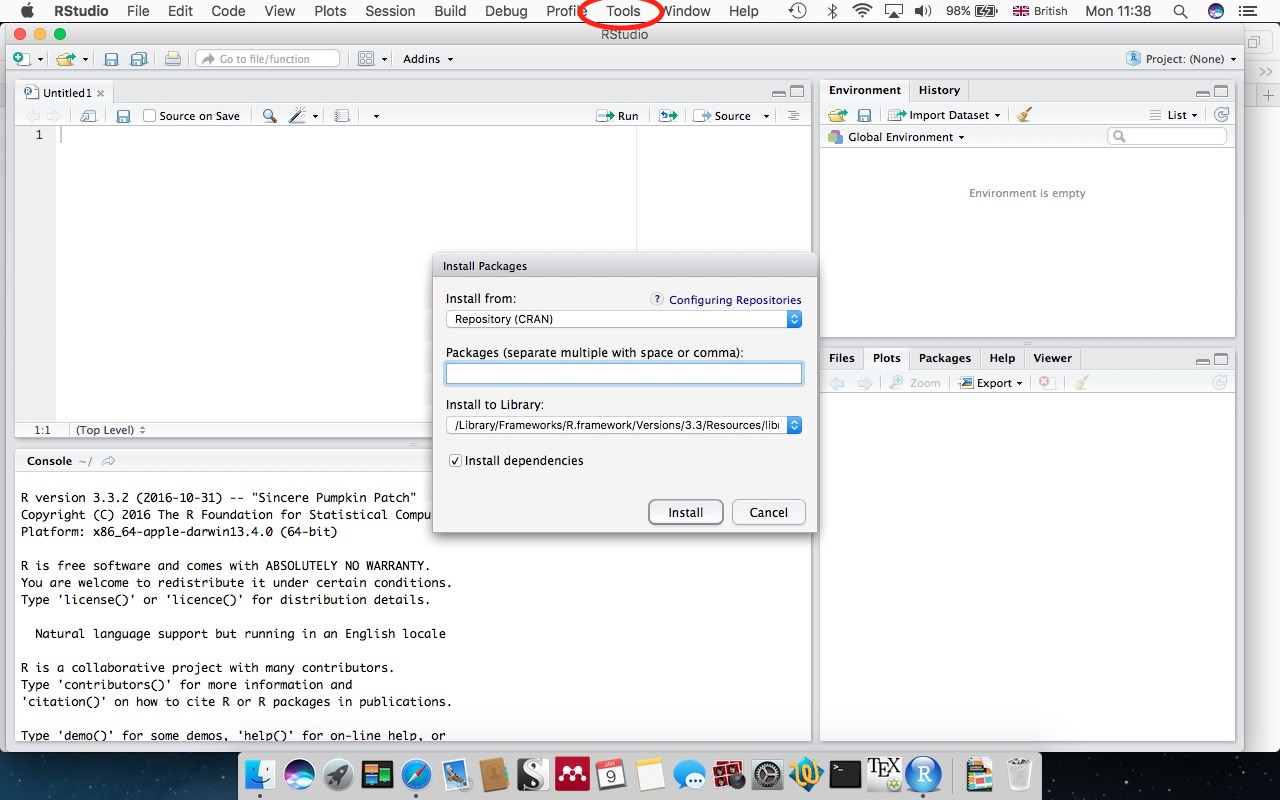
\includegraphics[width=0.75\textwidth]{installPkg.jpg}
	\caption{R Studio Install Packages}
\end{figure}

You will need to write the name of each package you wish to download separated by a comma or space. However, this will only work for packages which are available from the CRAN website. Alternatively, packages can be downloaded from the command line:
\medskip
\begin{minted}
[fontsize=\footnotesize,
linenos
]
{r} 
install.packages("name of package")
\end{minted}

It may take a little time for all the packages to install. Once this has been done, and the command prompt \textbf{\textgreater} is showing, you can continue. To load the packages you need to tell R you want to use them. We are going to use \textit{tm}, \textit{ggplot2} and \textit{wordcloud}.
\medskip
\begin{minted}
[fontsize=\footnotesize,
linenos
]
{r} 
library(tm) # tm is a text mining package
library(ggplot2) # ggplot2 is a graph plotting package
library(wordcloud) # lets you create wordclouds
\end{minted}

Now we have loaded the packages we want to use we need to load the corpus into R using the \textbf{tm} package. This will create a V or volatile corpus which means that it only exists in the current session of R. Next we will process the corpus removing punctuation, numbers, uppercase letters and white spaces. We could also remove stopwords, but we won't do that at the moment.
\medskip
\begin{minted}
[fontsize=\footnotesize,
linenos
]
{r} 
# load the corpus
docs <- Corpus(DirSource(dname)) 

# Preprocess the text
docs <- tm_map(docs, removePunctuation)   # Remove punctuation   
docs <- tm_map(docs, removeNumbers)      # Remove numbers    
docs <- tm_map(docs, tolower)   # Convert to lowercase   
# docs <- tm_map(docs, removeWords, stopwords("english")) # To remove stopwords 
docs <- tm_map(docs, stripWhitespace)   # Strip whitespace   
docs <- tm_map(docs, PlainTextDocument) 
# This is the end of the preprocessing stage.
\end{minted}

Once the corpus has been processed a Document Term Matrix (DTM) can be created. The DTM is a matrix which describes the frequency of terms in the corpus where each row is a document and each column is a word or term from the corpus.
\medskip
\begin{minted}
[fontsize=\footnotesize,
linenos
]
{r} 
# Create a Document Term Matrix
dtm <- DocumentTermMatrix(docs)   

# To view or export the DTM
corpus_dtm <- as.matrix(dtm)
rownames(corpus_dtm) <- c("PP", "MP")

# It is also possible to create a Term Document Matrix
tdm <- TermDocumentMatrix(docs)
corpus_tdm <- as.matrix(tdm)
colnames(corpus_tdm) <- c("PP", "MP")

# Write files to a folder
write.csv(corpus_dtm, "Results/dtm.csv")
write.csv(corpus_tdm, "Results/tdm.csv")

# Explore your data - this gives the raw frequency for each word in the corpus      
freq <- colSums(as.matrix(dtm))   
length(freq)   # the number of unique words in the corpus
head(freq) # view the top 6 elements
\end{minted}

It can be useful to visualise the word frequencies. Below are two examples, a frequency graph showing words which appear more than 500 times, and word clouds showing 100 words and words with a minimum frequency of 100.
\medskip
\begin{minted}
[fontsize=\footnotesize,
linenos
]
{r} 
# Create a frequency graph of the words which appear more than 500 times  
  
word_freq <- data.frame(word=names(freq), freq=freq)   
p <- ggplot(subset(word_freq, freq>500), aes(word, freq))    
p <- p + geom_bar(stat="identity")   
p <- p + theme(axis.text.x=element_text(angle=45, hjust=1))   
p  

# Create a wordcloud
  
set.seed(142)   # set.seed is used to ensure replicability
wordcloud(names(freq), freq, max.words=100)   

set.seed(142)   
wordcloud(names(freq), freq, min.freq=100, scale=c(5, .1), 
          colors=brewer.pal(8, "Set1"))  # This section determines the colours
\end{minted}

You could rerun the code on page 10 removing the \# at the start of line 8 to remove the stopwords to see the difference it makes to the visualisations.
 

\newpage
\section{Workshop Session Two: Word Vectors in R}

Session 2 is adapted from Benjamin Schmidt's (2015) blog post \href{http://bookworm.benschmidt.org/posts/2015-10-25-Word-Embeddings.html}{\textbf{Word Embeddings}} and my doctoral research 'Jane Austen in Vector Space' presented at JADH (2016), which can be found \href{https://sarajkerr.com/talks-and-papers/}{\textbf{here}}.

Begin by clearing your workspace, this can be done by clicking on the broom in the environment pane or choosing \textit{Session} - \textit{Clear Workspace}. This will remove all the objects created during the previous session.

\subsection{Create, or Load, a Vector Space Model}

The \textbf{wordVectors} package in R allows you to create a vector space model or to load a previously created model. The packages needed for this session should already have been loaded (see the Pre-workshop materials for details). 
\medskip
\begin{minted}
[fontsize=\footnotesize,
linenos
]
{r} 
# Install/load the packages needed for this session
install.packages("magrittr")
# If you are unable to install this package don't worry as I have included a 
# work around
 
library(wordVectors)
library(tsne)
library(Rtsne)
library(ggplot2)
library(ggrepel)
library(stringi)
library(magrittr) # only load this package if you have been able to install it
\end{minted}

Before a vector space model can be created the .txt files need to be processed. The \textbf{prep{\_}word2vec} function takes in a folder of .txt files and outputs a single .txt file which combines the texts in one document removes punctuation and converts all words to lower
case.  

The model then needs to be trained - this uses the skip-gram method of creating a vector space mode as default (the alternative is continuous bag of words), which is better for infrequent words. This tutorial (\href{https://www.tensorflow.org/tutorials/word2vec/}{\textbf{Vector Representations of Words}}) provides a detailed explanation of the difference between the two models.

The created model will appear in the environment pane in R Studio, a copy called \textbf{Novel.bin} will be saved to the \textit{Results} folder. This can be loaded into future R sessions saving processing time. It is important to remember that the larger the corpus the longer it will take to process and load.
\medskip
\begin{minted}
[fontsize=\footnotesize,
linenos
]
{r} 
# If a prepared text file has not already been created follow this step 

prep_word2vec("Austen_Texts/Novel_Files", "Austen_Texts/Novel_Files/
              Novel_corpus.txt", lowercase =  T)

# This can take some time depending on the size of the files

# train_word2vec takes several parameters - input prepared .txt file, an 
# output file, vectors are the number of dimensions the default is 100, and
# window is the number of words either side of the context word, by default
# the function uses the skip-gram method

ja <- train_word2vec("Austen_Texts/Novel_Files/Novel_corpus.txt", 
                          output = "Results/Novel.bin", threads = 3, 
                          vectors = 100, window = 15)

# This will take a little while to process
# A Vector Space Model has been created

# If a model has previously been created and saved it can be loaded using
ja <- read.vectors("Results/Novel.bin")
\end{minted}

\subsection{Prepare Texts for KWIC Analysis}

While the \textbf{wordVectors} package will allow a detailed exploration of the words from the corpus, it does not show the specific context in which the word originally appeared in the novel. To enable contextualisation of any words of interest, we will use the \textbf{kwic()} function we created in Session 1.
\medskip
\begin{minted}
[fontsize=\footnotesize,
linenos
]
{r} 
# Create a path to the files
input.dir <- "Austen_Texts/Novel_Files" 
# Read the name of all .txt files
files <- dir(input.dir, "\\.txt") 

# Create a function to list the files
show_files <- function(files){
        for(i in 1:length(files)){
                cat(i, files[i], "\n", sep = " ")
        }
}

# To use the function:
show_files(files) # the files are listed and numbered

# Create a function to create a list of words from each file, you will recognise
# the code from the previous sections

make_word_list <- function(files, input.dir) {
        # create an empty list for the results
        word_list <- list()
        # read in the files and process them
        for(i in 1:length(files)) {
                text <- scan(paste(input.dir, files[i], sep = "/"), 
                             what = "character", sep = "\n")   
                text <- paste(text, collapse = " ")
                text_lower <- tolower(text)
                text_words <- strsplit(text_lower, "\\W")
                text_words <- unlist(text_words)
                text_words <- text_words[which(text_words != "")]
                word_list[[files[i]]] <- text_words
        }
        return(word_list)
}


# To use the function:
my_corpus <- make_word_list(files, input.dir) 

# The Novel_corpus.txt file will be read in as 2 items as it has already been
# processed - this doesn't have an impact on using kwic() later.

# Creating a Key Word in Context (KWIC) function - this uses the output from
# the make_word_list and includes the show_files function 

kwic <- function(my_corpus) {
        show_files(names(my_corpus))
        # identify the chosen file
        file_id <- as.numeric(
              readline("Which file would you like to examine? Enter a number: \n"))
        # identifythe number of words each side of the keyword
        context <- as.numeric(
              readline("How much context do you want? Enter a number: \n"))
        # identify the focus word
        keyword <- tolower((readline("Enter a keyword: \n")))
        # create the KWIC readout
        hits <- which(my_corpus[[file_id]] == keyword)
        if(length(hits) > 0) {
                result <- NULL
                for(j in 1:length(hits)) {
                        start <- hits[j] - context
                        if(start < 1) {
                                start <- 1
                        }
                        end <- hits[j] + context
                        cat("\n--------------------", j, "----------------\n")
                        cat(my_corpus[[file_id]][start:(hits[j] -1)], sep = " ")
                        cat("[", my_corpus[[file_id]][hits[j]], "] ", sep = " ")
                        cat(my_corpus[[file_id]][(hits[j] +1): end], sep = " ")
                        myrow <- cbind(hits[j],
                                   paste(my_corpus[[file_id]][start: (hits[j] -1)],
                                             collapse = " "),
                                   paste(my_corpus[[file_id]][hits[j]],
                                             collapse = " "),
                                   paste(my_corpus[[file_id]][(hits[j] +1): end],
                                             collapse = " "))
                        result <- rbind(result, myrow)
                }
                colnames(result) <- c("position", "left", "keyword", "right")
                return(result)
        } else {
                cat("YOUR KEYWORD WAS NOT FOUND\n")
        }
}

# To use the function, this time there will be a choice of three files, 
# Pride and Prejudice, Mansfield Park, and a text combining the two:
results <- kwic(my_corpus)

\end{minted}

\subsection{Exploring a Vector Space Model}

There are a number of function built into the \textbf{wordVectors} package which allow the vector space model to be explored. We will look at the \textbf{nearest{\_}to()} function. Details of other functions can be found on the GitHub page for the \textbf{wordVectors} package - \href{https://github.com/bmschmidt/wordVectors}{\textbf{here}}.

The \textbf{nearest{\_}to()} function allows you to search the vector space model for words which appear near to a chosen word or set of words, both semantically and contextually. The selected words can be viewed as a list or a plot. It is useful at this point to explore the specific context any words of interest appear in by using the \textbf{kwic()} function.
\medskip
\begin{minted}
[fontsize=\footnotesize,
linenos
]
{r} 
# The nearest_to() function uses cosine similarity
nearest_to(ja, ja[["marriage"]], 50) # 50 nearest words to marriage

marriage <- nearest_to(ja, ja[["marriage"]], 100)
# This creates a vector of distances for the 100 words nearest to marriage

# Create a plot of the 100 words nearest to marriage       
plot(ja[[names(marriage), average = F]])  
# This takes a little time to run

wealth <- ja %>% nearest_to(ja[[c("establishment","income", "fortune",
                "privilege","wealth", "property", "affluence")]], 300) %>% names
# This uses the 'magrittr' package which acts as a pipeline enabling short cuts
# It works in a similar manner to the vector for marriage but extracts the names
sample(wealth, 100) 
# This allows a random sample of 100 words to be taken from the vector

# If you were not able to install 'magrittr' the same result can be created by 
# using the following code:

wealth1 <- nearest_to(ja, ja[[c("establishment","income", "fortune",
                "privilege","wealth", "property", "affluence")]], 300)

wealth1 <- names(wealth1)

sample(wealth1, 100)

# Plot the chosen segment
plot(ja[[wealth[1:100], average = F]])

# using the kwic() function explore the context of some of the words in the
# plot
results1 <- kwic(my_corpus)

# If you wish to save your results amend this piece of code:
# If you wish to save the results as a .csv file
write.csv(results, "Results/yourkeyword_text.csv")

\end{minted}


\subsection{Using the w2v{\_}analysis Function}

To speed up the exploration of the vector space model I created a function called \textbf{w2v{\_}analysis} using the \textbf{wordVectors} package but plotting in \textbf{ggplot2} which allows more modifications. This function uses the \textbf{Rtsne} package which uses the Barnes-Hut implementation of T-sne and is somewhat quicker than the \textbf{tsne} package which is used in the \textbf{plot()} function in \textbf{wordVectors}. 
\medskip
\begin{minted}
[fontsize=\footnotesize,
linenos
]
{r} 
# The function takes 4 arguments:
# vsm - a vector space model 
# words - a character vector of focus words
# seed - an integer
# path - the path to the folder you want files saved to 
# ref_name - the reference name for the exported files 

# The function will create a vector which is the average of the words input and 
# will output a wordlist of the 500 nearest words, a csv of the words and their
# positions, and a plot of the 2D reduction of the vector space
# model using the Barnes-Hut implementation of t-SNE. The points for each word
# are marked in red so the labels can be moved by ggrepel for ease of reading.
# set.seed is used to ensure replicability

w2v_analysis <- function(vsm, words, seed, path, ref_name) {
        # Set the seed
        if (!missing(seed))
                set.seed(seed)
        
        # Identify the nearest 10 words to the average vector of search terms
        ten <- nearest_to(vsm, vsm[[words]])
        
        # Identify the nearest 500 words to the average vector of search terms and 
        # save as a .txt file
        main <- nearest_to(vsm, vsm[[words]], 500)
        wordlist <- names(main)
        filepath <- paste0(path, ref_name)
        write(wordlist, paste0(filepath, ".txt"))
        
        
        # Create a subset vector space model
        new_model <- vsm[[wordlist, average = F]]
        
        # Run Rtsne to reduce new VSM to 2D (Barnes-Hut)
        reduction <- Rtsne(as.matrix(new_model), dims = 2, initial_dims = 50, 
                           perplexity = 30, theta = 0.5, check_duplicates = F,
                           pca = F, max_iter = 1000, verbose = F, 
                           is_distance = F, Y_init = NULL)
        
        # Extract Y (positions for plot) as a dataframe and add row names
        df <- as.data.frame(reduction\$Y)
        rows <- rownames(new_model)
        rownames(df) <- rows
        
        # Save dataframe as .csv file
        write.csv(df, paste0(filepath, ".csv"))
        
        # Create t-SNE plot and save as jpeg
        ggplot(df) +
                geom_point(aes(x = V1, y = V2), color = "red") +
                geom_text_repel(aes(x = V1, y = V2, label = rownames(df))) +
                xlab("Dimension 1") +
                ylab("Dimension 2 ") +
                # geom_text(fontface = 2, alpha = .8) +
                theme_bw(base_size = 12) + 
                theme(legend.position = "none") +
                ggtitle(paste0("2D reduction of VSM ", ref_name," using t_SNE"))
        
        ggsave(paste0(ref_name, ".jpeg"), path = path, width = 24, 
               height = 18, dpi = 100)
        
        new_list <- list("Ten nearest" = ten, "Status" = "Analysis Complete") 
        return(new_list)
        
}

# To use the function a single word or a vector of connected words can be used
status <- c("status", "rank", "position", "superior", "aristocracy", "gentry")

# The function is called as below:
# w2v_analysis(VectorSpaceModel, Word, Number, "Path/", "Reference_Name")
# E.g.
w2v_analysis(ja, status, 42, "Results/", "Status")

\end{minted}

This will take a short time to run. The console will return the 10 nearest words and include the status "Analysis Complete". If you look in the Results folder there will be 3 new files a .txt file containing the word list of the 500 nearest words, a csv containing the words and their position in the plot, and a .jpeg file containing the plot. 

Take some time to explore the model.

\subsection{Some Resources on using word2vec with Asian Texts}
Here are some resources and articles on using word2vec with Asian texts.
\begin{itemize}
 \item \href{http://www.iaiai.org/journals/index.php/IEE/article/download/20/35}{\textbf{Vector Similarity of Related Words and Synonyms in the Japanese WordNet}}.
 \item \href{http://www.itdadao.com/articles/c19a338733p0.html}{\textbf{Japanese-words-to-vectors: Word2vec (word to vectors) approach for Japanese language using Gensim}}.
 \item \href{http://ai.stanford.edu/~wzou/emnlp2013_ZouSocherCerManning.pdf}{\textbf{Bilingual Word Embeddings for Phrase-Based Machine Translation}}.
 \end{itemize} 
 
 \newpage
 
 \section{Contact Details}
 If you wish to contact me my details are:
 \begin{itemize}
 \item \textbf{Email:} sarajkerr@icloud.com
 \item \textbf{Web:} \url{http://sarajkerr.com}
 \item \textbf{Twitter:} @data{\_}fiend
 \item \textbf{GitHub:} \url{https://github.com/SaraJKerr}
 \end{itemize}
\end{document}